\chapter{МОДЕЛИРОВАНИЕ РОСТА ТРЕЩИН АВТОГРП В ДЛИНУ} \label{ch4}

\section{Постановка задачи}
\vspace*{-5mm}

На основе модели одномерных утечек Картера \cite{karter} в работе \cite{koning} получена первая формула Кёнинга, которая представляет собой зависимость полудлины трещины автоГРП от расхода жидкости, фильтрационно-ёмкостных свойств (ФЕС) пласта, репрессии на пласт и времени:
\beq\label{Koning_first}
x_{\!f}=\frac{Q\mu\sqrt{\pi\kappa t}}{2\pi k_eh\left(p_{\!f}-p_e\right)},
\eeq
где $Q$ -- расход нагнетаемой в рассматриваемую трещину жидкости;
$\mu$ -- вязкость жидкости;
$\kappa=k_e/(\varphi_e\mu c_t)$ -- коэффициент пьезопроводности пласта;
$t$ -- время закачки;
$k_e$ -- проницаемость пласта;
$\varphi_e$ -- пористость пласта;
$c_t$ -- общая сжимаемость системы (состоит из сжимаемости флюидов и сжимаемости порового пространства);
$h$ -- эффективная толщина (мощность) пласта;
$\Delta p=p_{\!f}-p_e$ -- разница между средним давлением в трещине и пластовым давлением (репрессия на пласт).\\

В текущей работе рассматривается одновременный рост нескольких трещин гидроразрыва, поэтому расход жидкости на каждой из них может динамично меняться согласно правилам Кирхгофа.
Кроме того, давление в трещинах в общем случае тоже может меняться по мере увеличения объёма трещин и изменения расхода на них.
Получается, что согласно формуле \eqref{Koning_first} есть зависимость полудлины трещины $x_{\!f}$ от расхода на трещине $Q$, но при этом на расход в общем случае может влиять текущая полудлина каждой из трещин.

Таким образом, для корректного применения формулы Кёнинга приращение полудлины каждой из трещин на текущем шаге по времени необходимо найти как произведение полной производной формулы Кёнинга по времени и рассматриваемого временного шага.\newline
Полная производная полудлины трещины $x_{\!f}$ по времени $t$:
\beq\label{FullDerivative}
\frac{dx_{\!f}}{dt}=\frac{\partial x_{\!f}}{\partial t}+\frac{\partial x_{\!f}}{\partial Q}\frac{dQ}{dt}+\frac{\partial x_{\!f}}{\partial (p_{\!f}-p_e)}\frac{d(p_{\!f}-p_e)}{dt}
\eeq
Частная производная полудлины трещины $x_{\!f}$ по времени $t$:
\beq\label{PartialDerivative_t_first}
\frac{\partial x_{\!f}}{\partial t}=\frac{Q\mu}{4\pi k_eh\left(p_{\!f}-p_e\right)}\sqrt{\frac{\pi\kappa}{t}}
\eeq
Частная производная полудлины трещины $x_{\!f}$ по расходу $Q$:
\beq\label{PartialDerivative_Q_first}
\frac{\partial x_{\!f}}{\partial Q}=\frac{\mu\sqrt{\pi\kappa t}}{2\pi k_eh\left(p_{\!f}-p_e\right)}
\eeq
Частная производная полудлины трещины $x_{\!f}$ по репрессии на пласт $\left(p_{\!f}-p_e\right)$:
\beq\label{PartialDerivative_p_first}
\frac{\partial x_{\!f}}{\partial (p_{\!f}-p_e)}=-\frac{Q\mu\sqrt{\pi\kappa t}}{2\pi k_eh\left(p_{\!f}-p_e\right)^2}
\eeq
Подставляя \eqref{PartialDerivative_t_first}, \eqref{PartialDerivative_Q_first} и \eqref{PartialDerivative_p_first} в выражение \eqref{FullDerivative}, получаем:
\beq\label{FullDerivativeExplicit_first}
\frac{dx_{\!f}}{dt}=\frac{\mu}{2\pi k_e h(p_{\!f}-p_e)}\left(\frac{Q}{2}\sqrt{\frac{\pi\kappa}{t}}+\sqrt{\pi\kappa t}\,\frac{dQ}{dt}-\frac{Q\sqrt{\pi\kappa t}}{\left(p_{\!f}-p_e\right)}\frac{d(p_{\!f}-p_e)}{dt}\right)
\eeq
             
Итак, приращение полудлины трещины на каждом шаге по времени при рассмотрении случая одномерных утечек Картера записывается в следующем виде:
\beq\label{IncrementExplicit_first}
dx_{\!f}=\frac{\mu}{2\pi k_e h(p_{\!f}-p_e)}\left(\frac{Q}{2}\sqrt{\frac{\pi\kappa}{t}}dt+\sqrt{\pi\kappa t}\,dQ-\frac{Q\sqrt{\pi\kappa t}}{\left(p_{\!f}-p_e\right)}d(p_{\!f}-p_e)\right)
\eeq\\

Дополнительно в работе \cite{koning} получена вторая формула Кёнинга, которая применяется в случае двумерных радиальных утечек жидкости из трещины в пласт и представляет собой зависимость полудлины трещины автоГРП от расхода жидкости, фильтрационно-ёмкостных свойств (ФЕС) пласта, репрессии на пласт и времени:
\beq\label{Koning_second}
x_{\!f}=3\exp{\!\left(-\frac{2\pi k_e h\left(p_{\!f}-p_e\right)}{Q\mu}\right)}\sqrt{\kappa t}
\eeq
В этом случае частная производная полудлины трещины $x_{\!f}$ по времени $t$:
\beq\label{PartialDerivative_t_second}
\frac{\partial x_{\!f}}{\partial t}=\frac{3}{2}\exp{\left(-\frac{2\pi k_e h \left(p_{\!f}-p_e\right)}{Q\mu}\right)}\sqrt{\frac{\kappa}{t}}
\eeq
Частная производная полудлины трещины $x_{\!f}$ по расходу $Q$:
\beq\label{PartialDerivative_Q_second}
\frac{\partial x_{\!f}}{\partial Q}=\frac{6\pi k_e h\left(p_{\!f}-p_e\right)}{Q^2\mu}\exp{\!\left(-\frac{2\pi k_e h\left(p_{\!f}-p_e\right)}{Q\mu}\right)}\sqrt{\kappa t}
\eeq
Частная производная полудлины трещины $x_{\!f}$ по репрессии на пласт $\left(p_{\!f}-p_e\right)$:
\beq\label{PartialDerivative_p_second}
\frac{\partial x_f}{\partial (p_{\!f}-p_e)}=-\frac{6\pi k_e h}{Q\mu}\exp{\!\left(-\frac{2\pi k_e h\left(p_{\!f}-p_e\right)}{Q\mu}\right)}\sqrt{\kappa t}
\eeq

Подставляя \eqref{PartialDerivative_t_second}, \eqref{PartialDerivative_Q_second} и \eqref{PartialDerivative_p_second} в выражение \eqref{FullDerivative}, получаем:
\beq
\begin{gathered}
\frac{dx_{\!f}}{dt}=\exp{\!\left(-\frac{2\pi k_e h\left(p_{\!f}-p_e\right)}{Q\mu}\right)}\left(\frac{3}{2}\sqrt{\frac{\kappa}{t}}\,+\right.\\[10pt]
+\left.\frac{6\pi k_e h\left(p_{\!f}-p_e\right)}{Q^2\mu}\sqrt{\kappa t}\,\frac{dQ}{dt}-\frac{6\pi k_e h}{Q\mu}\sqrt{\kappa t}\,\frac{d(p_{\!f}-p_e)}{dt}\right)
\end{gathered}
\eeq

Итак, приращение полудлины трещины на каждом шаге по времени при рассмотрении случая двумерных радиальных утечек жидкости из трещины в пласт записывается в следующем виде:
\beq\label{IncrementExplicit_second}
\begin{gathered}
dx_{\!f}=\exp{\!\left(-\frac{2\pi k_e h\left(p_{\!f}-p_e\right)}{Q\mu}\right)}\left(\frac{3}{2}\sqrt{\frac{\kappa}{t}}dt\,+\right.\\[10pt]
+\left.\frac{6\pi k_e h\left(p_{\!f}-p_e\right)}{Q^2\mu}\sqrt{\kappa t}\,dQ-\frac{6\pi k_e h}{Q\mu}\sqrt{\kappa t}\,d(p_{\!f}-p_e)\right)
\end{gathered}
\eeq

Постановка задачи принимает следующий вид: используя решатель уравнений Кирхгофа, реализованный в главе \ref{ch3}, и формулы для приращения полудлины трещины \eqref{IncrementExplicit_first} и \eqref{IncrementExplicit_second}, построить графики зависимостей полудлины трещины и расхода на трещинах от времени при одномерных утечках Картера и при двумерных радиальных утечках жидкости из трещины в пласт.

\section{Описание численного алгоритма решения}
\vspace*{-5mm}

На рис. \ref{fig:koning_scheme} представлен алгоритм, по которому проводилось моделирование роста трещин автоГРП в длину.

\begin{figure}[H] 
\center
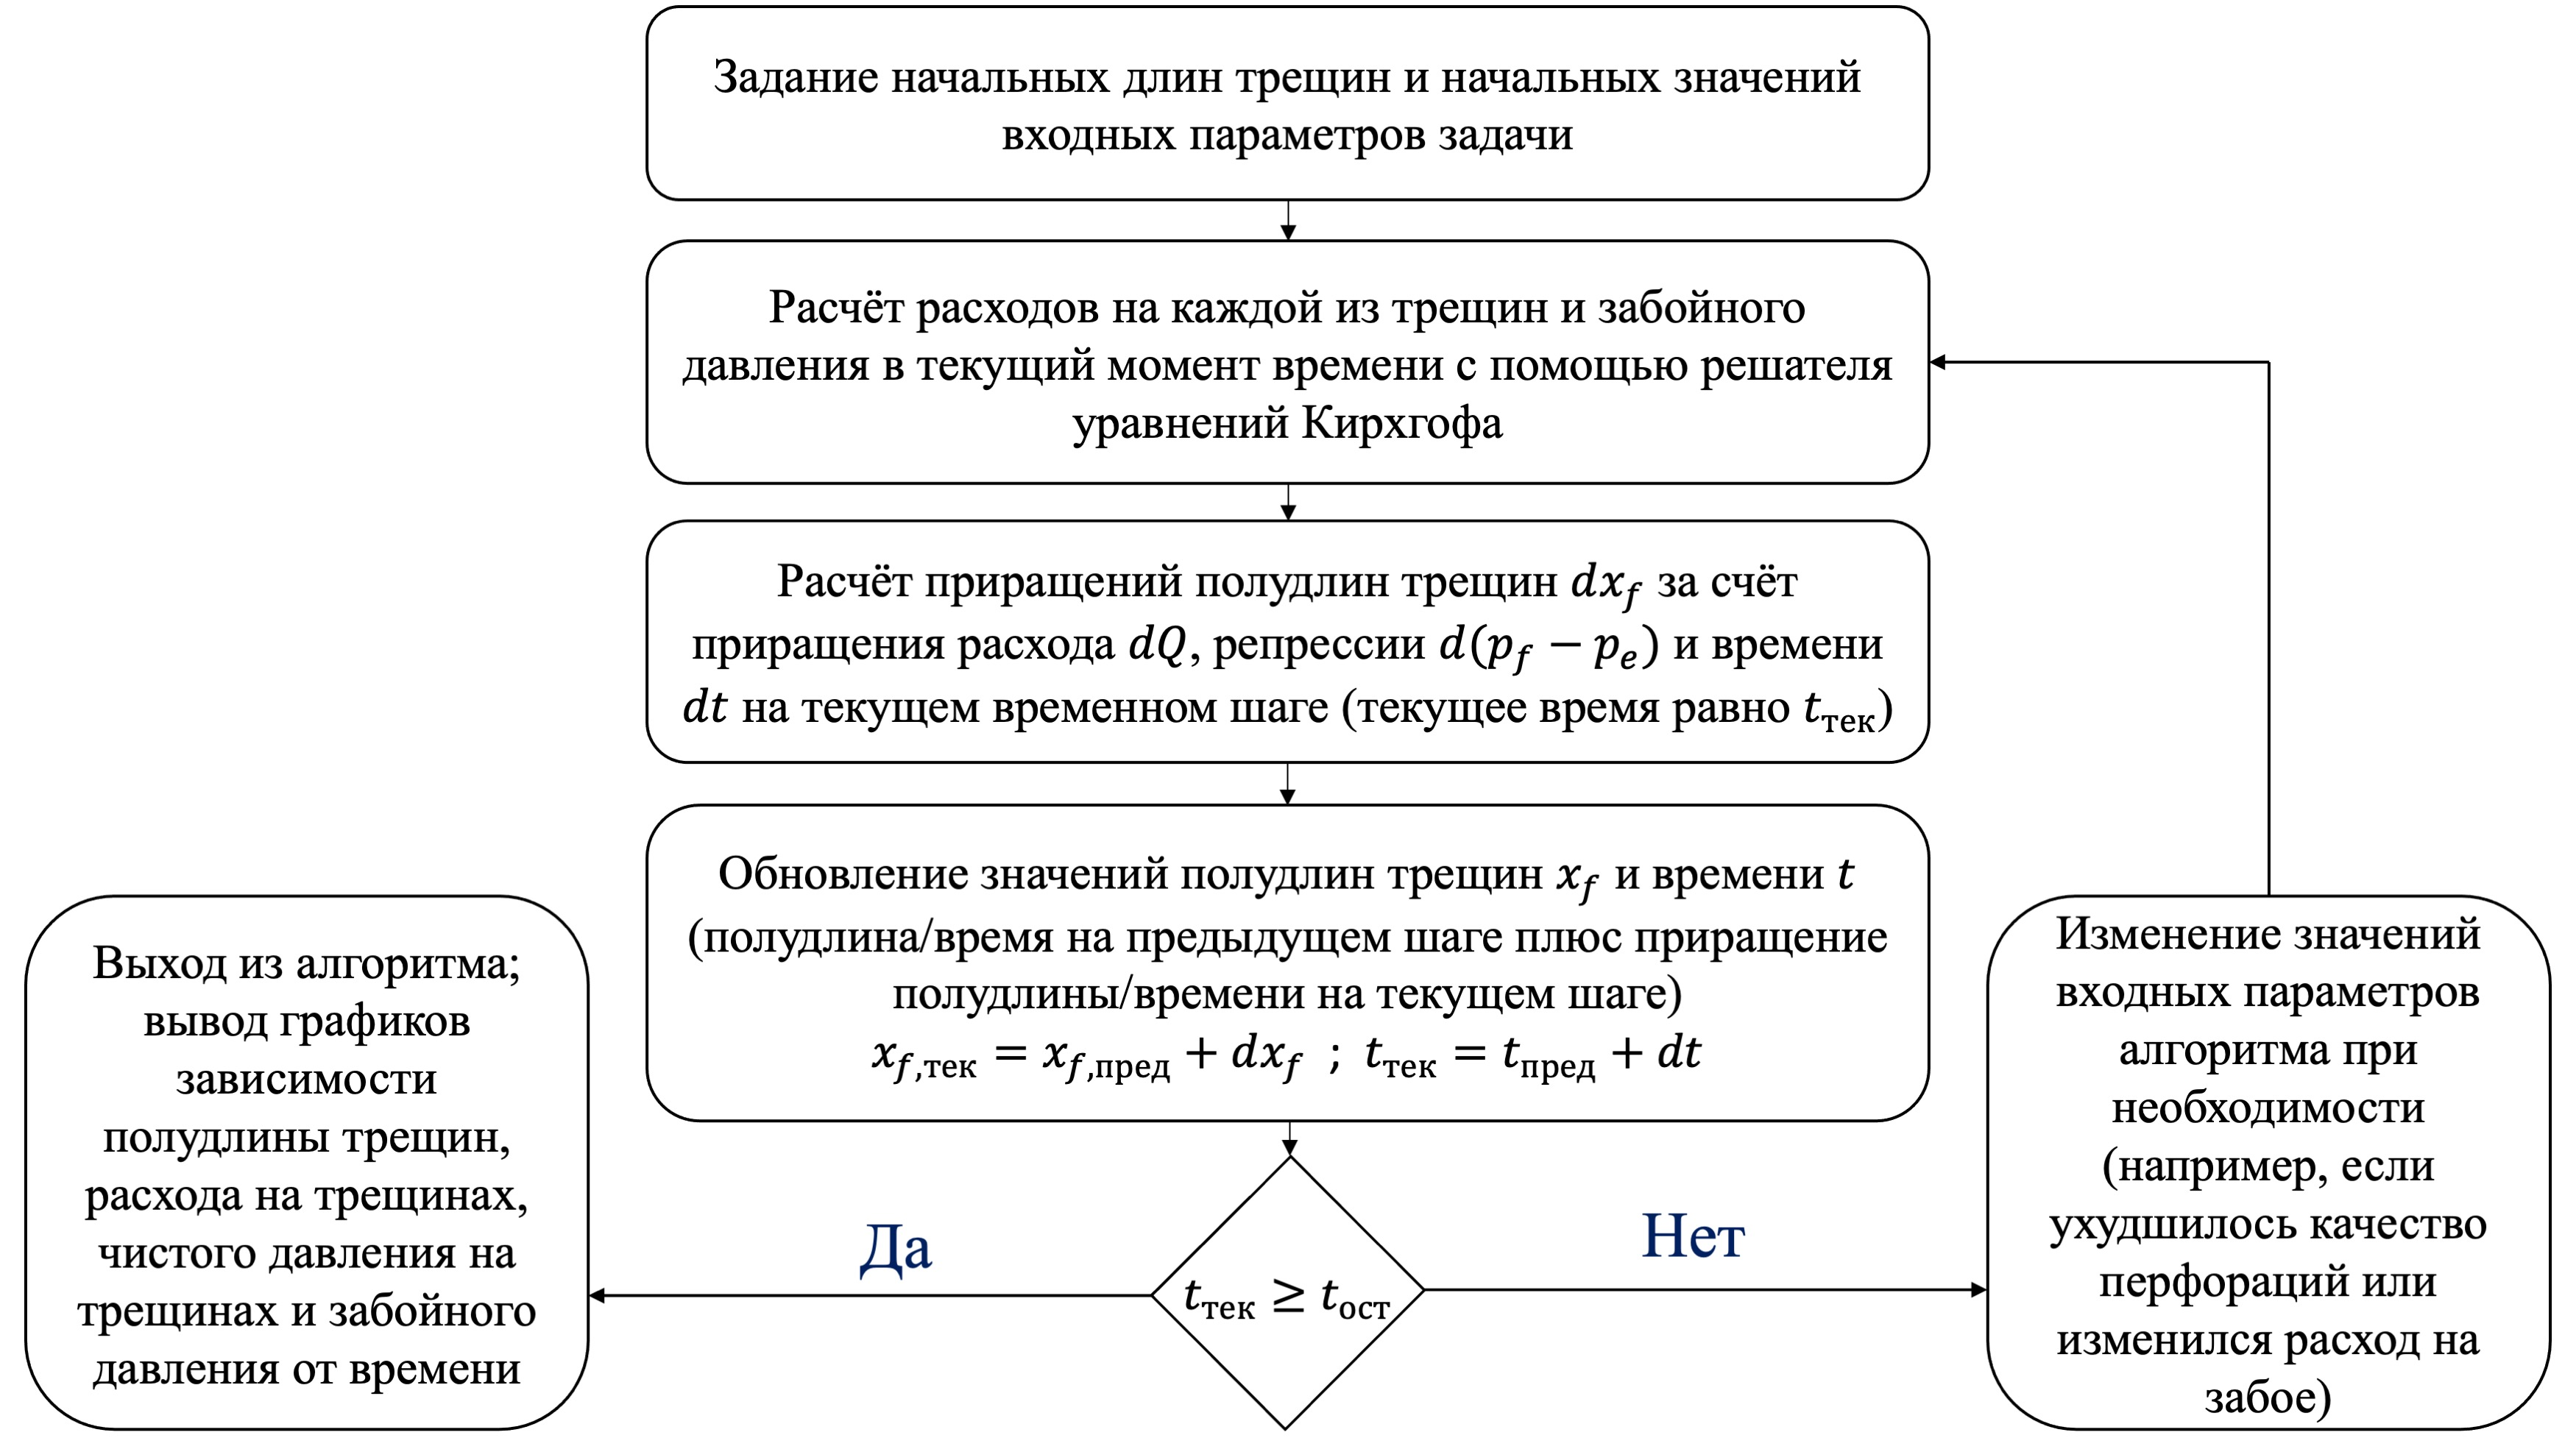
\includegraphics[width=\linewidth]{images/Koning_scheme.jpg}
\caption{Алгоритм расчёта полудлин трещин в зависимости от времени} 
\label{fig:koning_scheme}
\end{figure}

Совмещение формулы Кёнинга с уравнениями Кирхгофа будет проведено следующим образом:

1) на текущем шаге по времени по имеющимся значениям полудлины трещин автоГРП предыдущего шага будут рассчитаны давления и расходы на каждой трещине;

2) на основе полученных значений приращения давления и расхода будет найдено приращение полудлины трещины $dx_{\!f}$ на данном временном шаге по формуле \eqref{IncrementExplicit_first} в случае одномерных утечек Картера и по формуле \eqref{IncrementExplicit_second} в случае двумерных радиальных утечек жидкости из трещины в пласт;

3) по формуле $x_{\!f}^{\text{current}}=x_{\!f}^{\text{last}}+dx_{\!f}$ будут найдены полудлины каждой из трещин на текущем временном шаге;

4) описанные действия будут проделаны до требуемого шага по времени (условия остановки).

\section{Результаты моделирования}
\vspace*{-5mm}

Значения входных параметров, выбранные перед запуском алгоритма представлены в таблице \ref{tab:input-parameters-for-fractures-growth}.

\newcolumntype{L}[1]{>{\raggedright\arraybackslash}m{#1}}
\newcolumntype{C}[1]{>{\centering\arraybackslash}p{#1}}
\noindent % for correct centering
\begingroup
\small %выставляем шрифт в 12bp
\begin{longtable}[l]{|C{8cm}|C{8cm}|}
	\caption{Значения входных параметров алгоритма расчёта полудлины трещин}%
	\label{tab:input-parameters-for-fractures-growth}% label всегда желательно идти после caption
	\\
	\hline
	\multicolumn{1}{|c|}{\textbf{Параметр}}&\multicolumn{1}{|c|}{\textbf{Значение}}\\ \hline
	\endfirsthead%
	\captionsetup{format=tablenocaption,labelformat=continued} % до caption!
	\caption[]{}\\ % печать слов о продолжении таблицы
	\hline
	\multicolumn{1}{|c|}{\textbf{Параметр}}&\multicolumn{1}{|c|}{\textbf{Значение}}\\ \hline
	\endhead
	\hline
	\endfoot
	\hline
	\endlastfoot
	Расход на забое $Q_0$&1000 м$^3$/сут\\ \hline
	Вязкость закачиваемой жидкости (воды) $\mu$ & $10^{-3}$ Па$\cdot$с\\ \hline
	Плотность закачиваемой жидкости (воды) $\rho$ & 1000 кг/м$^3$\\ \hline
	Проницаемость пласта $k_e$ & 1 мД\\ \hline
	Пористость пласта $\varphi_e$ & 0.2\\ \hline
	Общая сжимаемость $c_t$ & $2.2\cdot 10^{-9}$ Па$^{-1}$\\ \hline
	Пластовое давление $p_e$ & 25 МПа\\ \hline
	Модуль плоской деформации породы $E'$ & $10^4$ МПа\\ \hline
	Мощность (высота) пласта $H$ & 15 м\\ \hline
	Количество перфораций $n_p$ & 32\\ \hline
	Диаметр перфораций $d_p$ & 0.02 м\\ \hline
	Безразмерный коэффициент эрозии $C_d$ & 0.5\\ \hline
	Радиус участков трубы $R$ & 0.08 м\\ \hline
	Длина участков трубы $L$ & 100 м\\ \hline
	Давление смыкания $\sigma_{\text{min}}$ & 40 МПа\\ \hline
	Трещиностойкость породы $K_{Ic}$ & $10^6$ Па$\cdot$м$^{1/2}$\\ \hline
	Количество трещин & 4\\ \hline
\end{longtable}
\normalsize% возвращаем шрифт к нормальному
\endgroup

На рис. представлены результаты при базовых значениях параметров в случае одномерных утечек Картера.
Видим, что потоки на трещинах постоянны и длина трещины растёт согласно первой формуле Кёнинга \eqref{Koning_first}.

\begin{figure}[H] 
\center
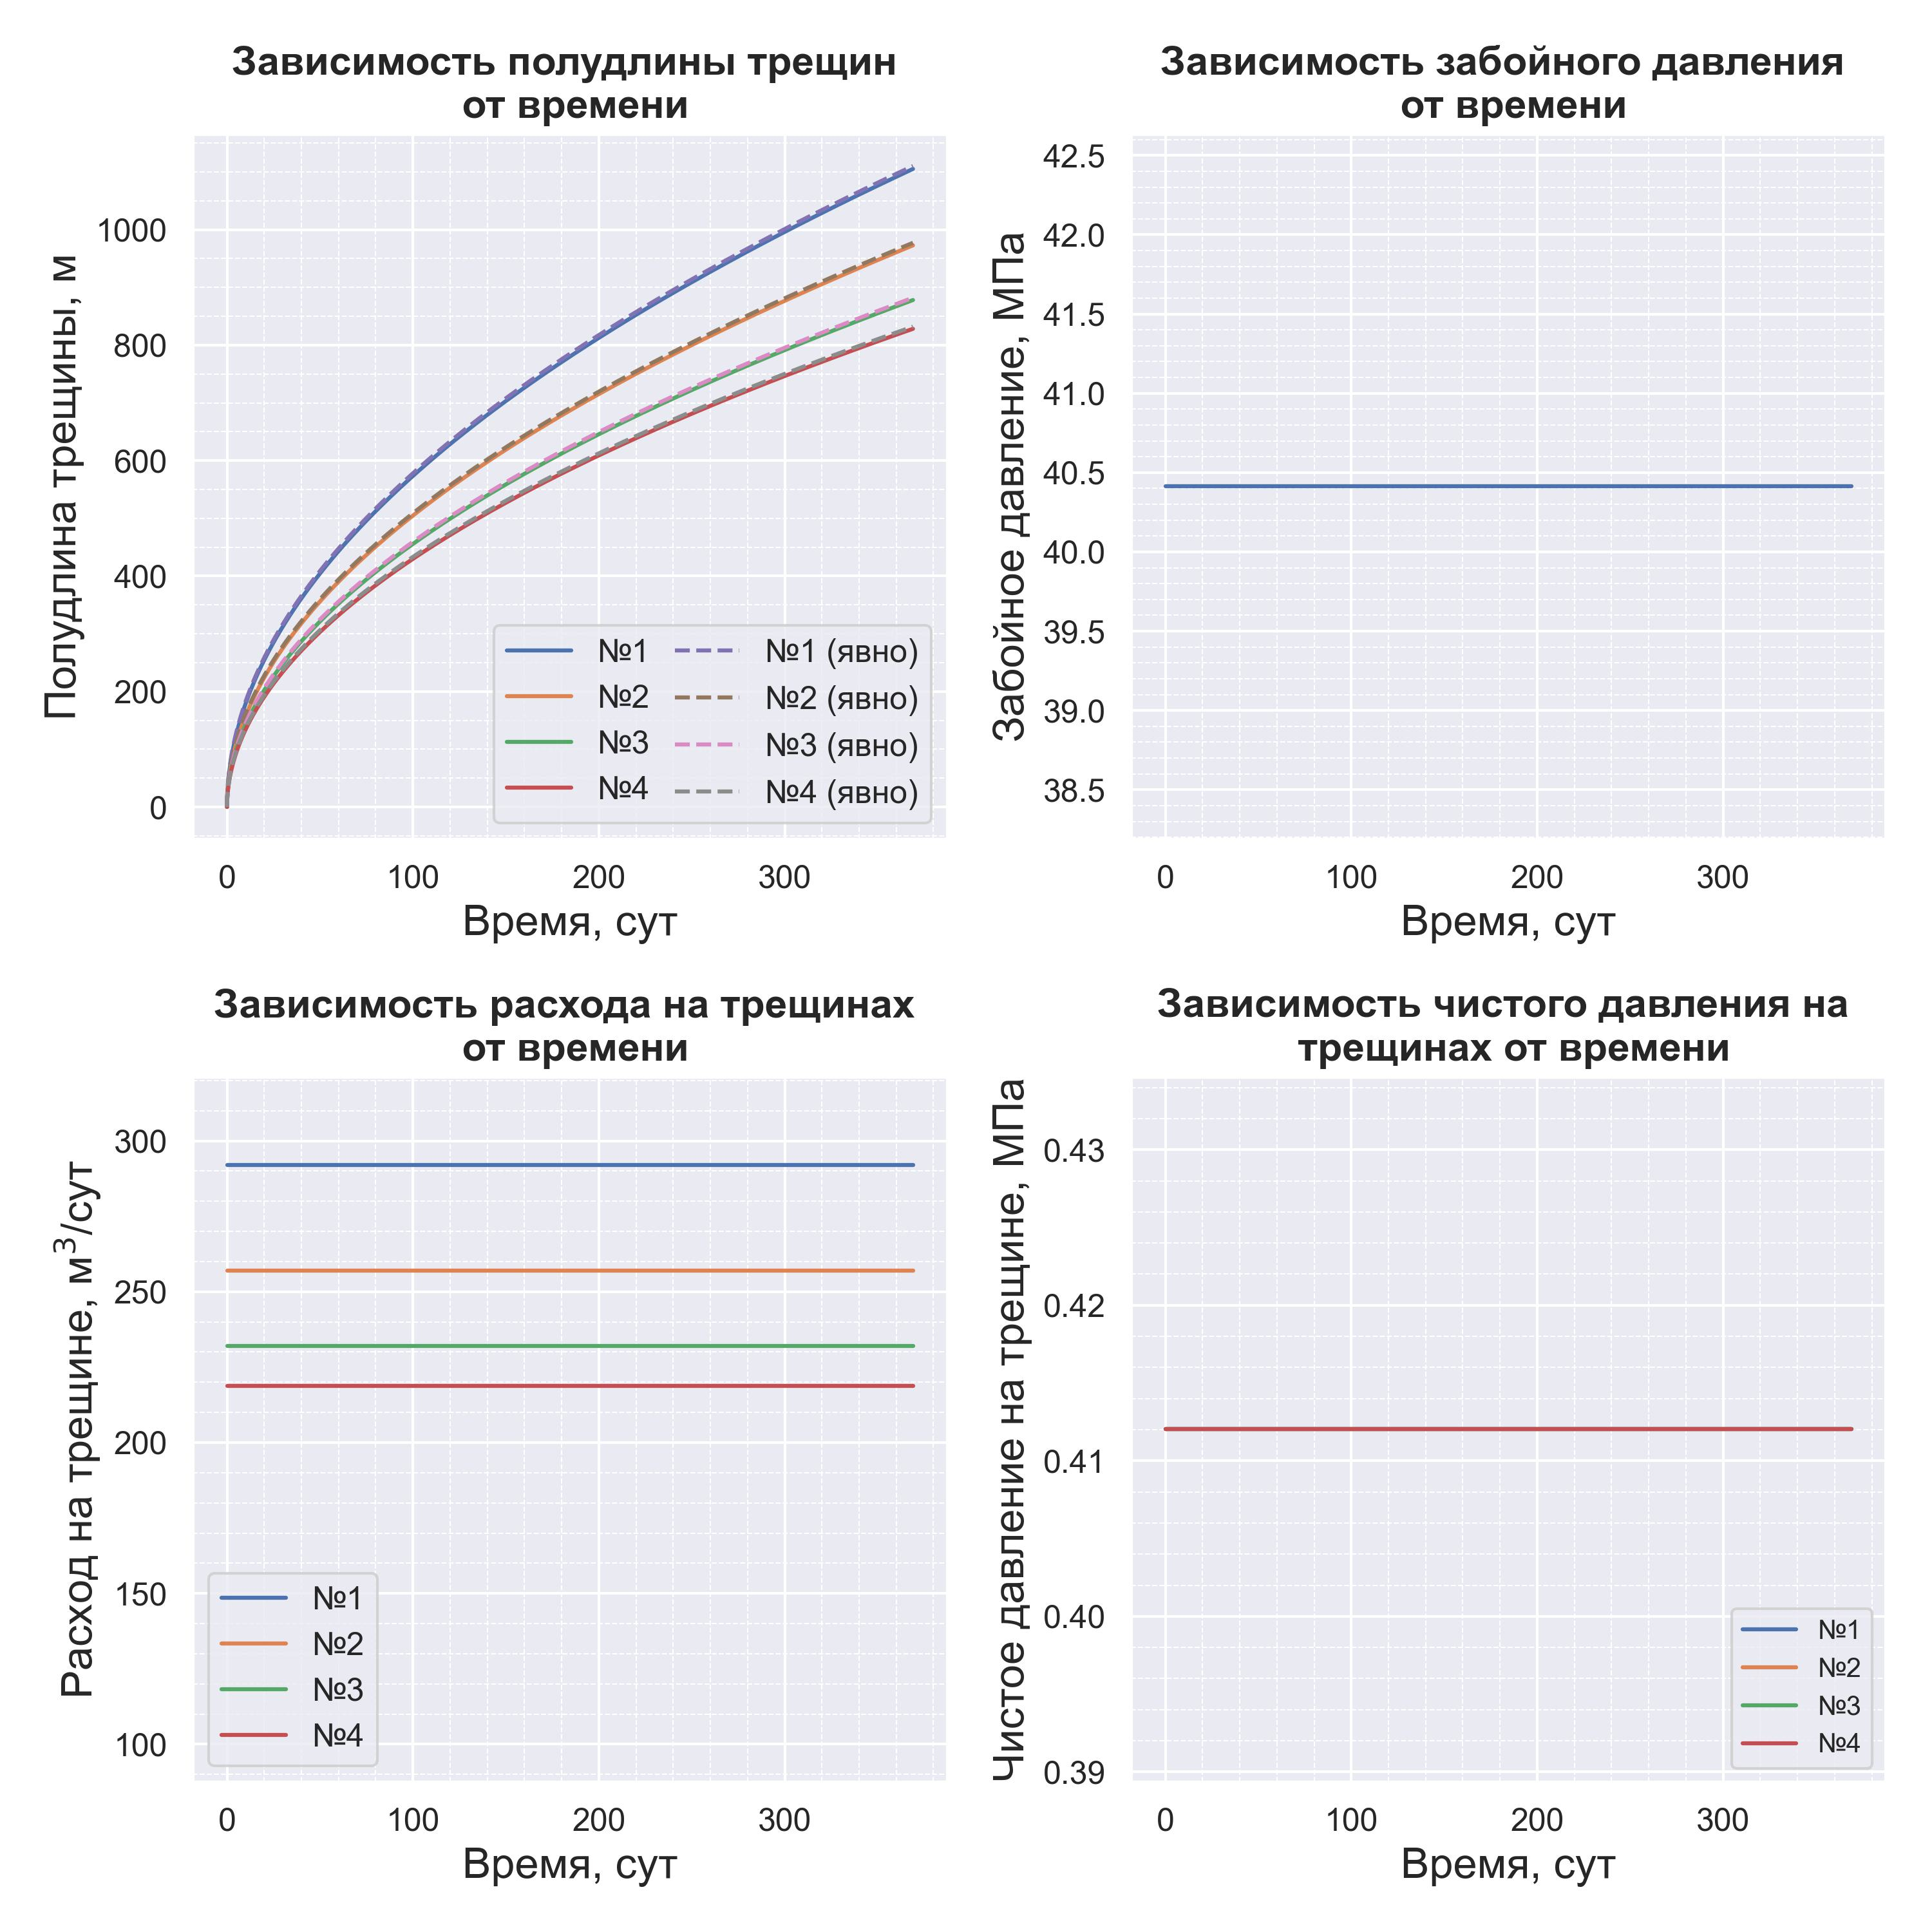
\includegraphics[width=\linewidth]{images/myimage1.jpg}
\caption{В случае одномерных утечек Картера и базовых параметрах алгоритма} 
\label{fig:myimage1}
\end{figure}

Такой же эксперимент проведён при двумерных радиальных утечках из трещины в пласт.
В этом случае трещины растут по второй формуле Кёнинга \eqref{Koning_second} и их длина в каждый момент времени меньше, чем длина, полученная в случае одномерных утечек Картера, что согласуется с результатами работы \cite{hagoort}.

\begin{figure}[H] 
\center
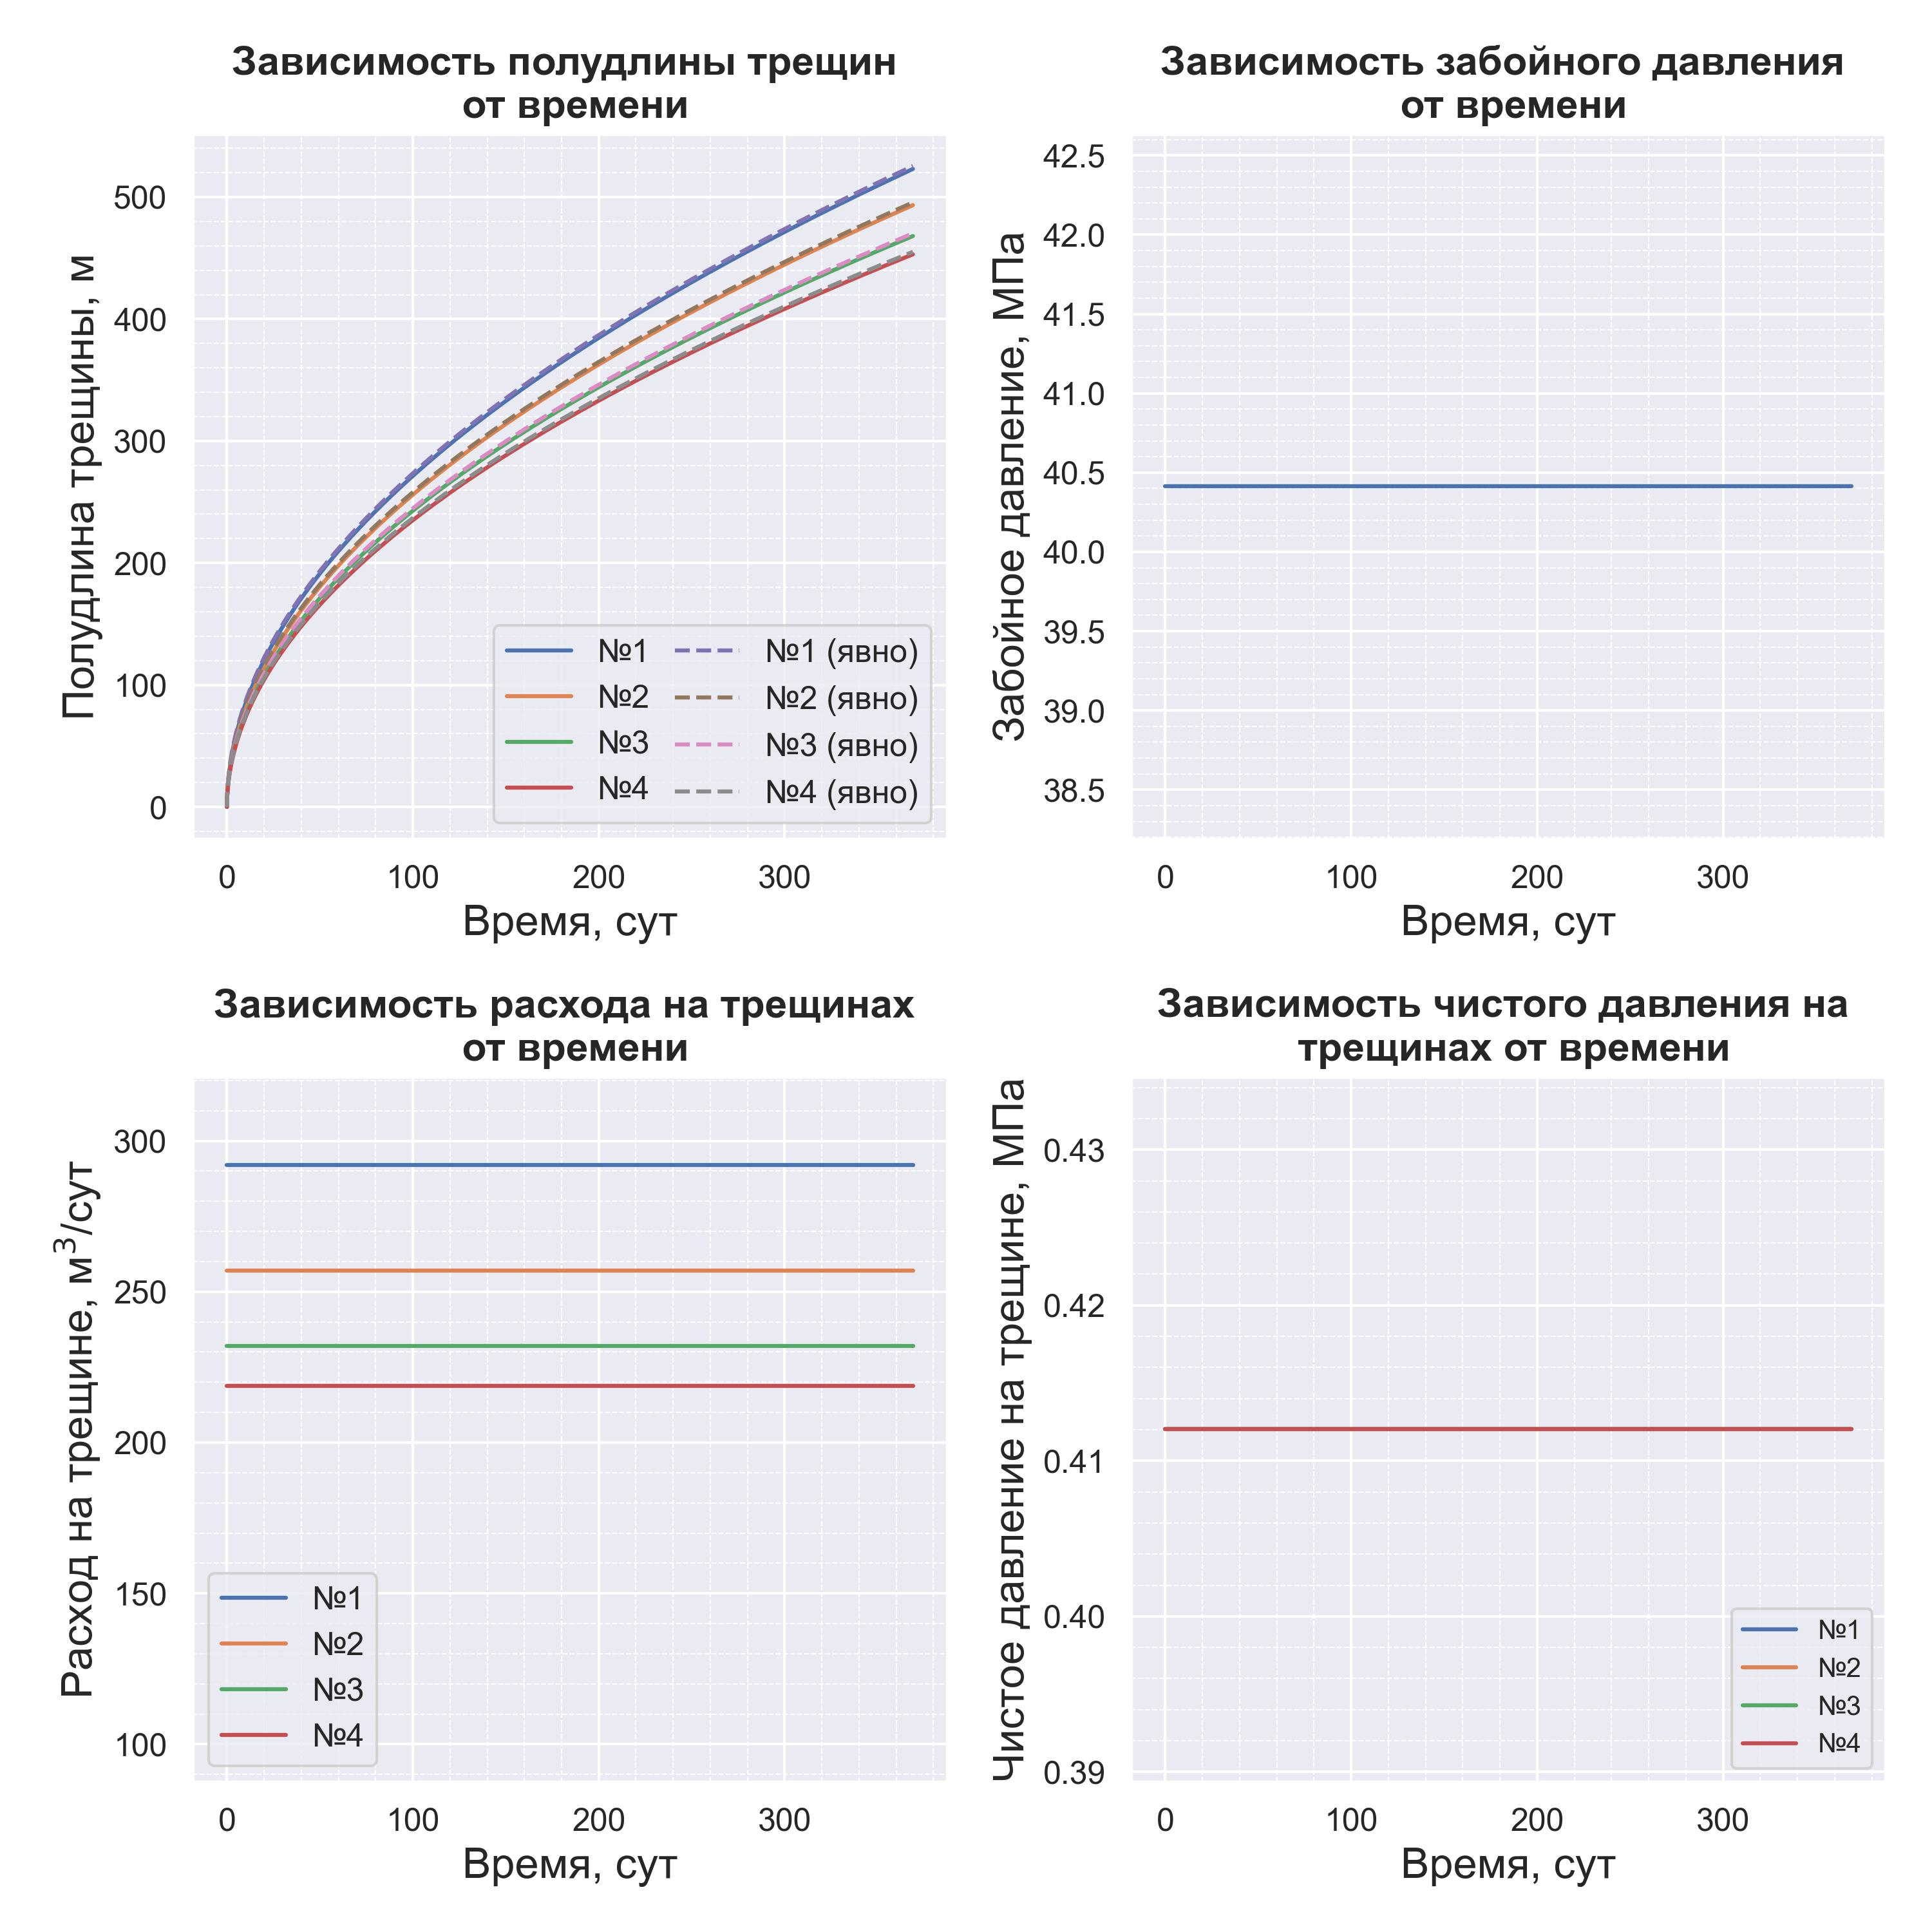
\includegraphics[width=\linewidth]{images/myimage2.jpg}
\caption{В случае двумерных радиальных утечек жидкости из трещины в пласт и базовых параметрах алгоритма} 
\label{fig:myimage2}
\end{figure}


Таким образом, предположение одномерности утечек по Картеру \cite{karter} может завышать оценку для длины растущих трещин автоГРП.


На рис. представлен эксперимент при периодическом изменении расхода жидкости на забое скважины.

\begin{figure}[H] 
\center
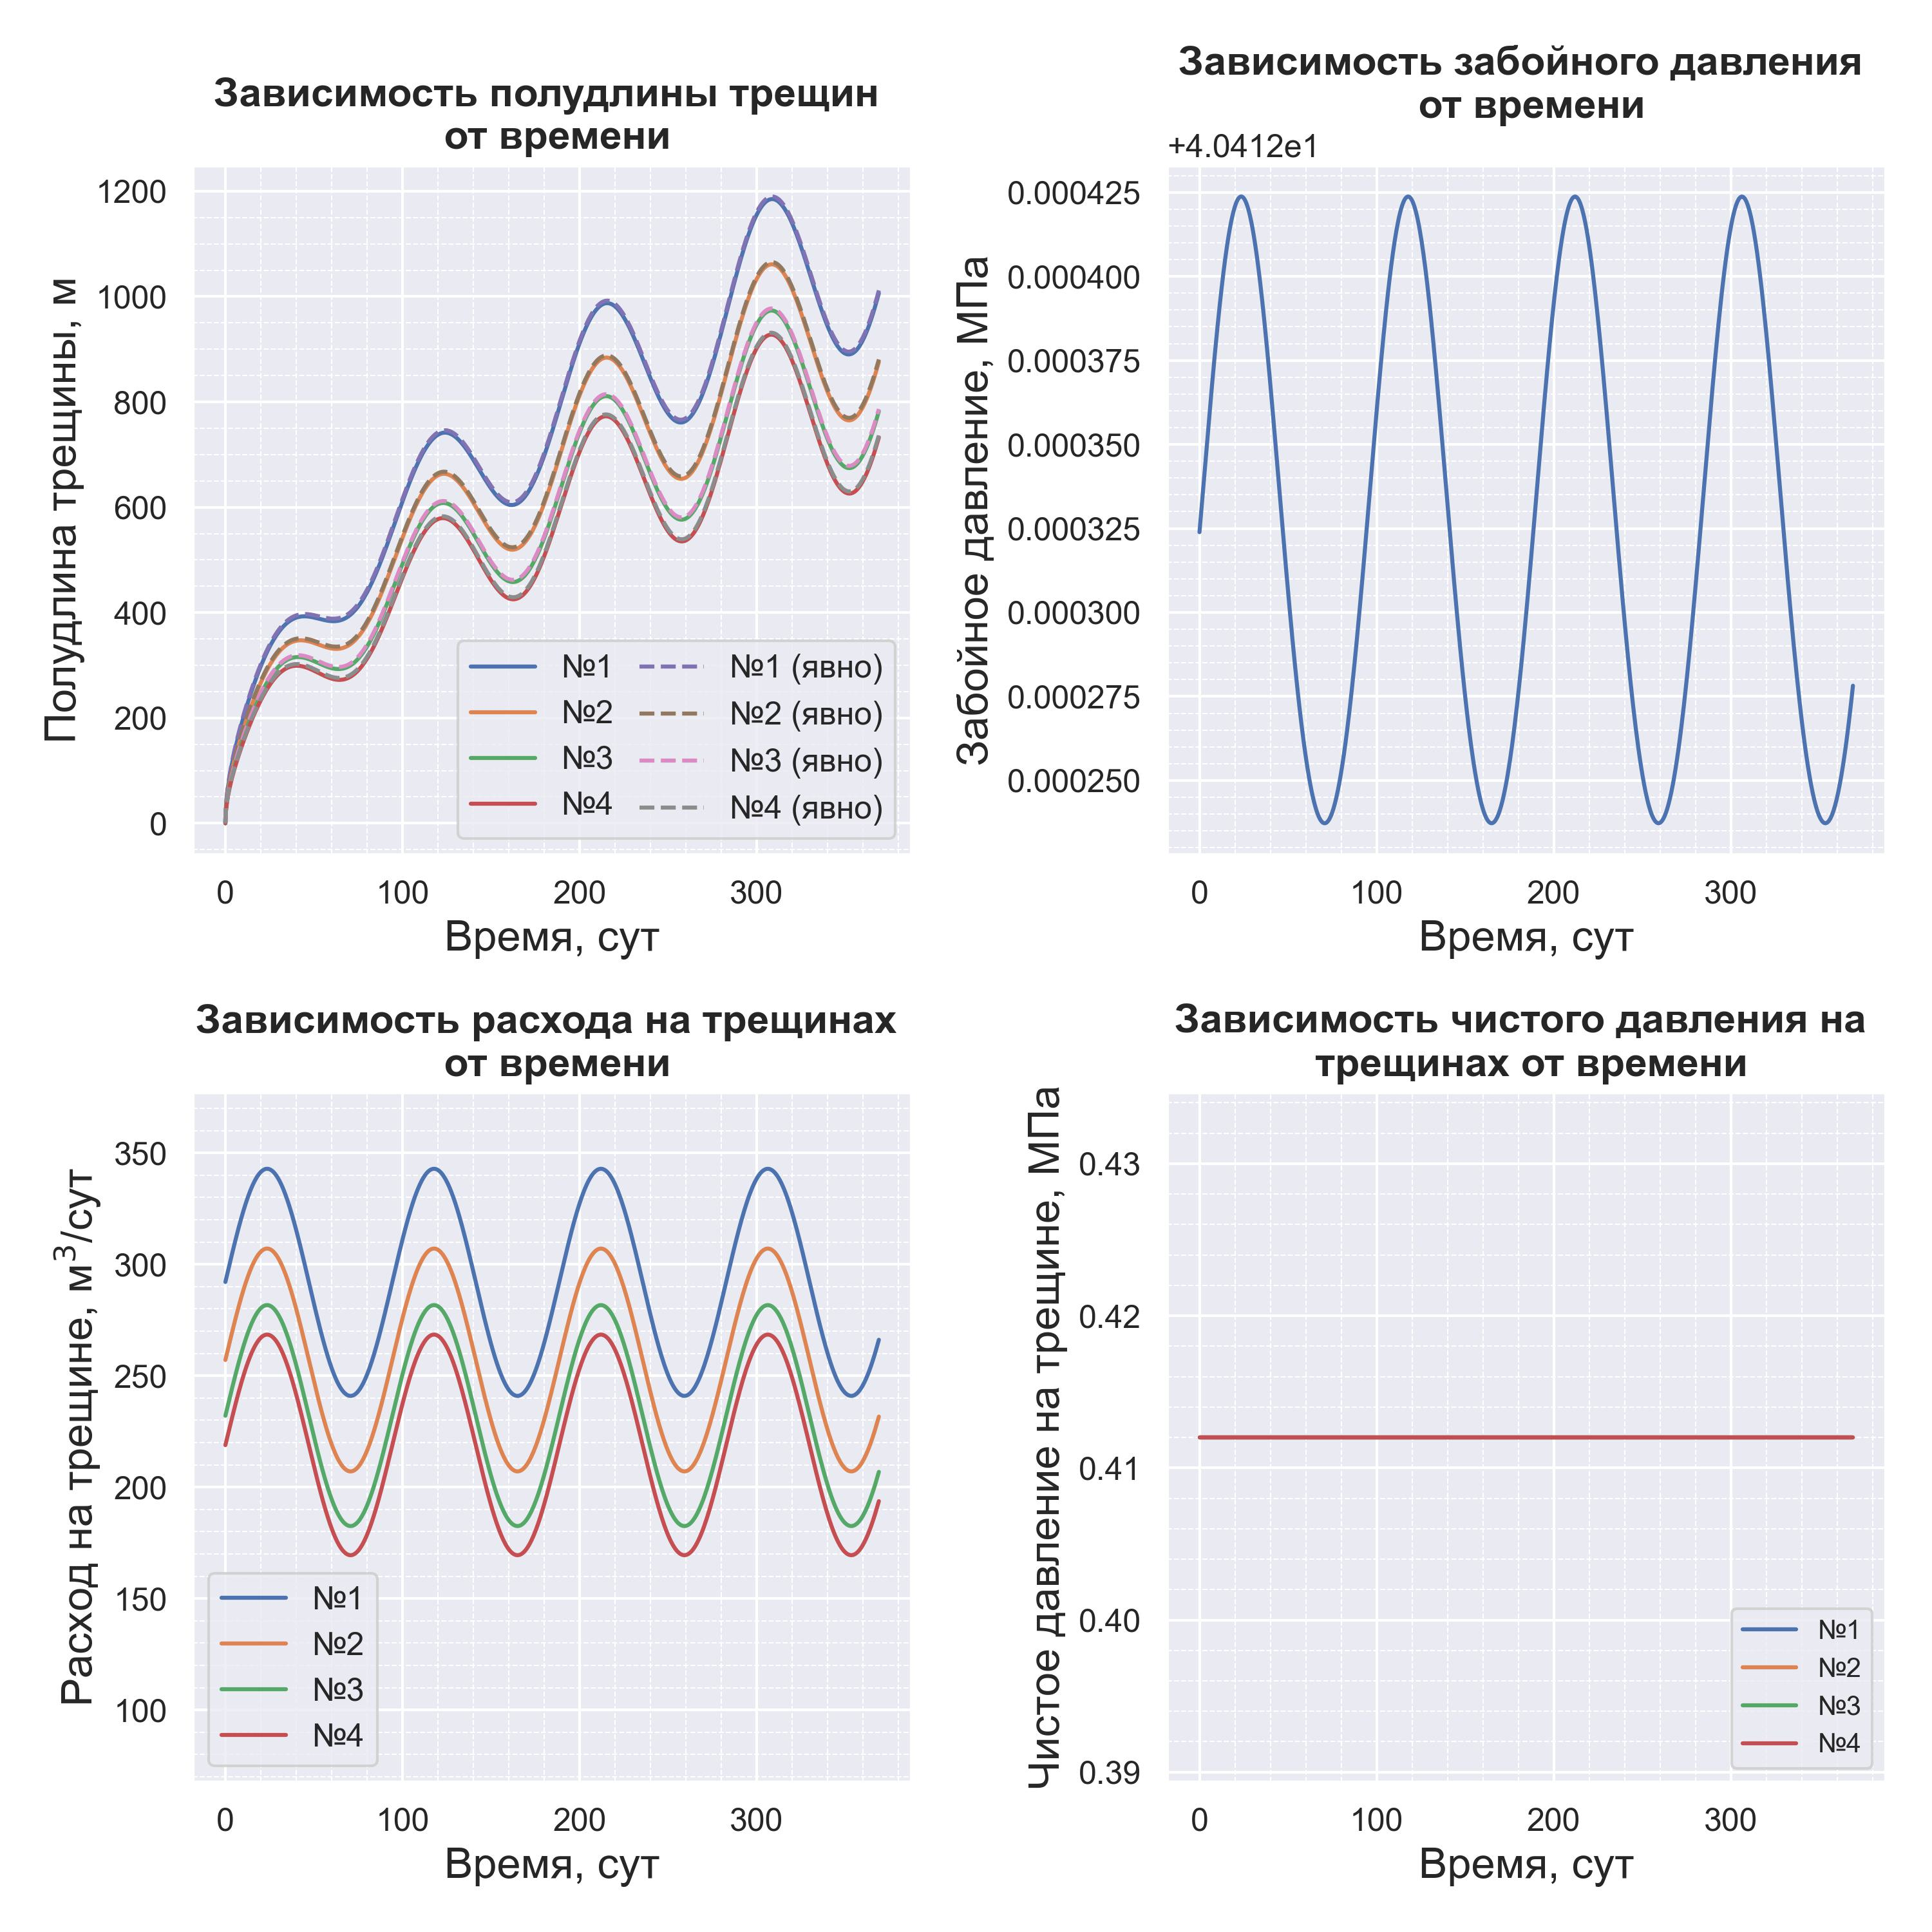
\includegraphics[width=\linewidth]{images/myimage3.jpg}
\caption{В случае одномерных утечек Картера и периодическом изменении расхода жидкости на забое скважины} 
\label{fig:myimage3}
\end{figure}


\begin{figure}[H] 
\center
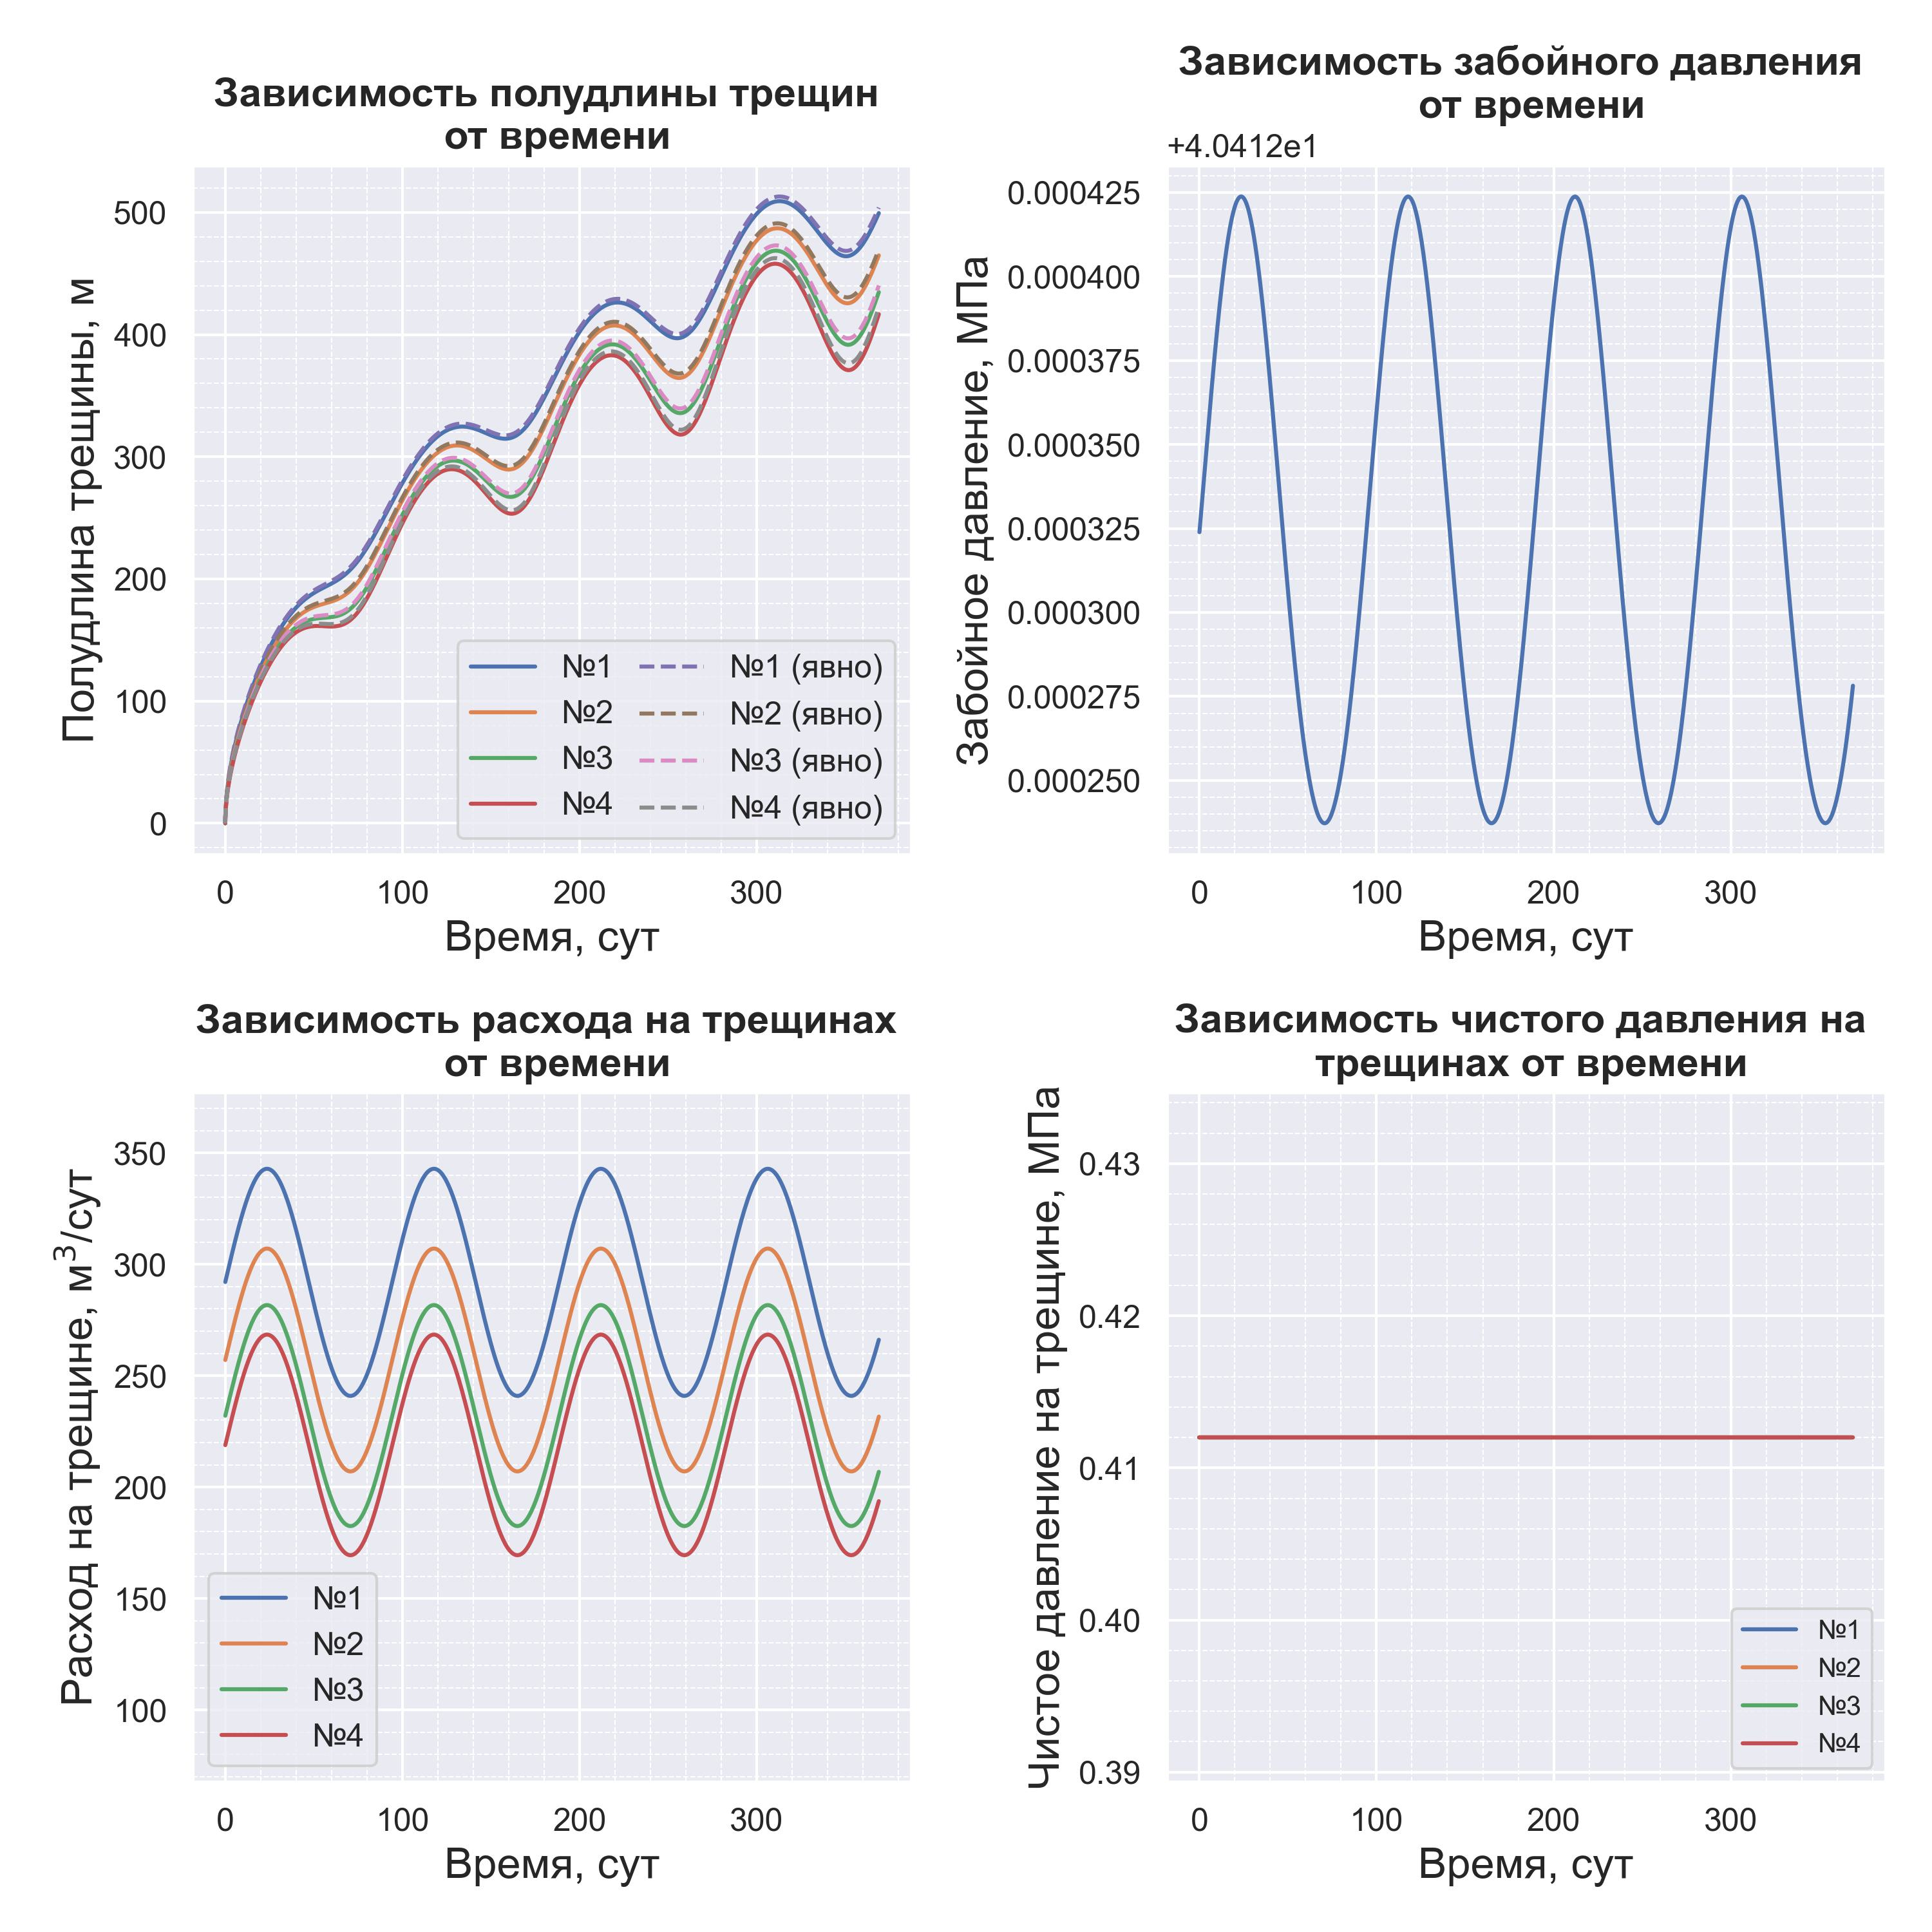
\includegraphics[width=\linewidth]{images/myimage4.jpg}
\caption{В случае двумерных радиальных утечек жидкости из трещины в пласт и периодическом изменении расхода жидкости на забое скважины}
\label{fig:myimage4}
\end{figure}


На рис. представлены результаты в случае линейного уменьшения расхода жидкости на забое скважины.

\begin{figure}[H] 
\center
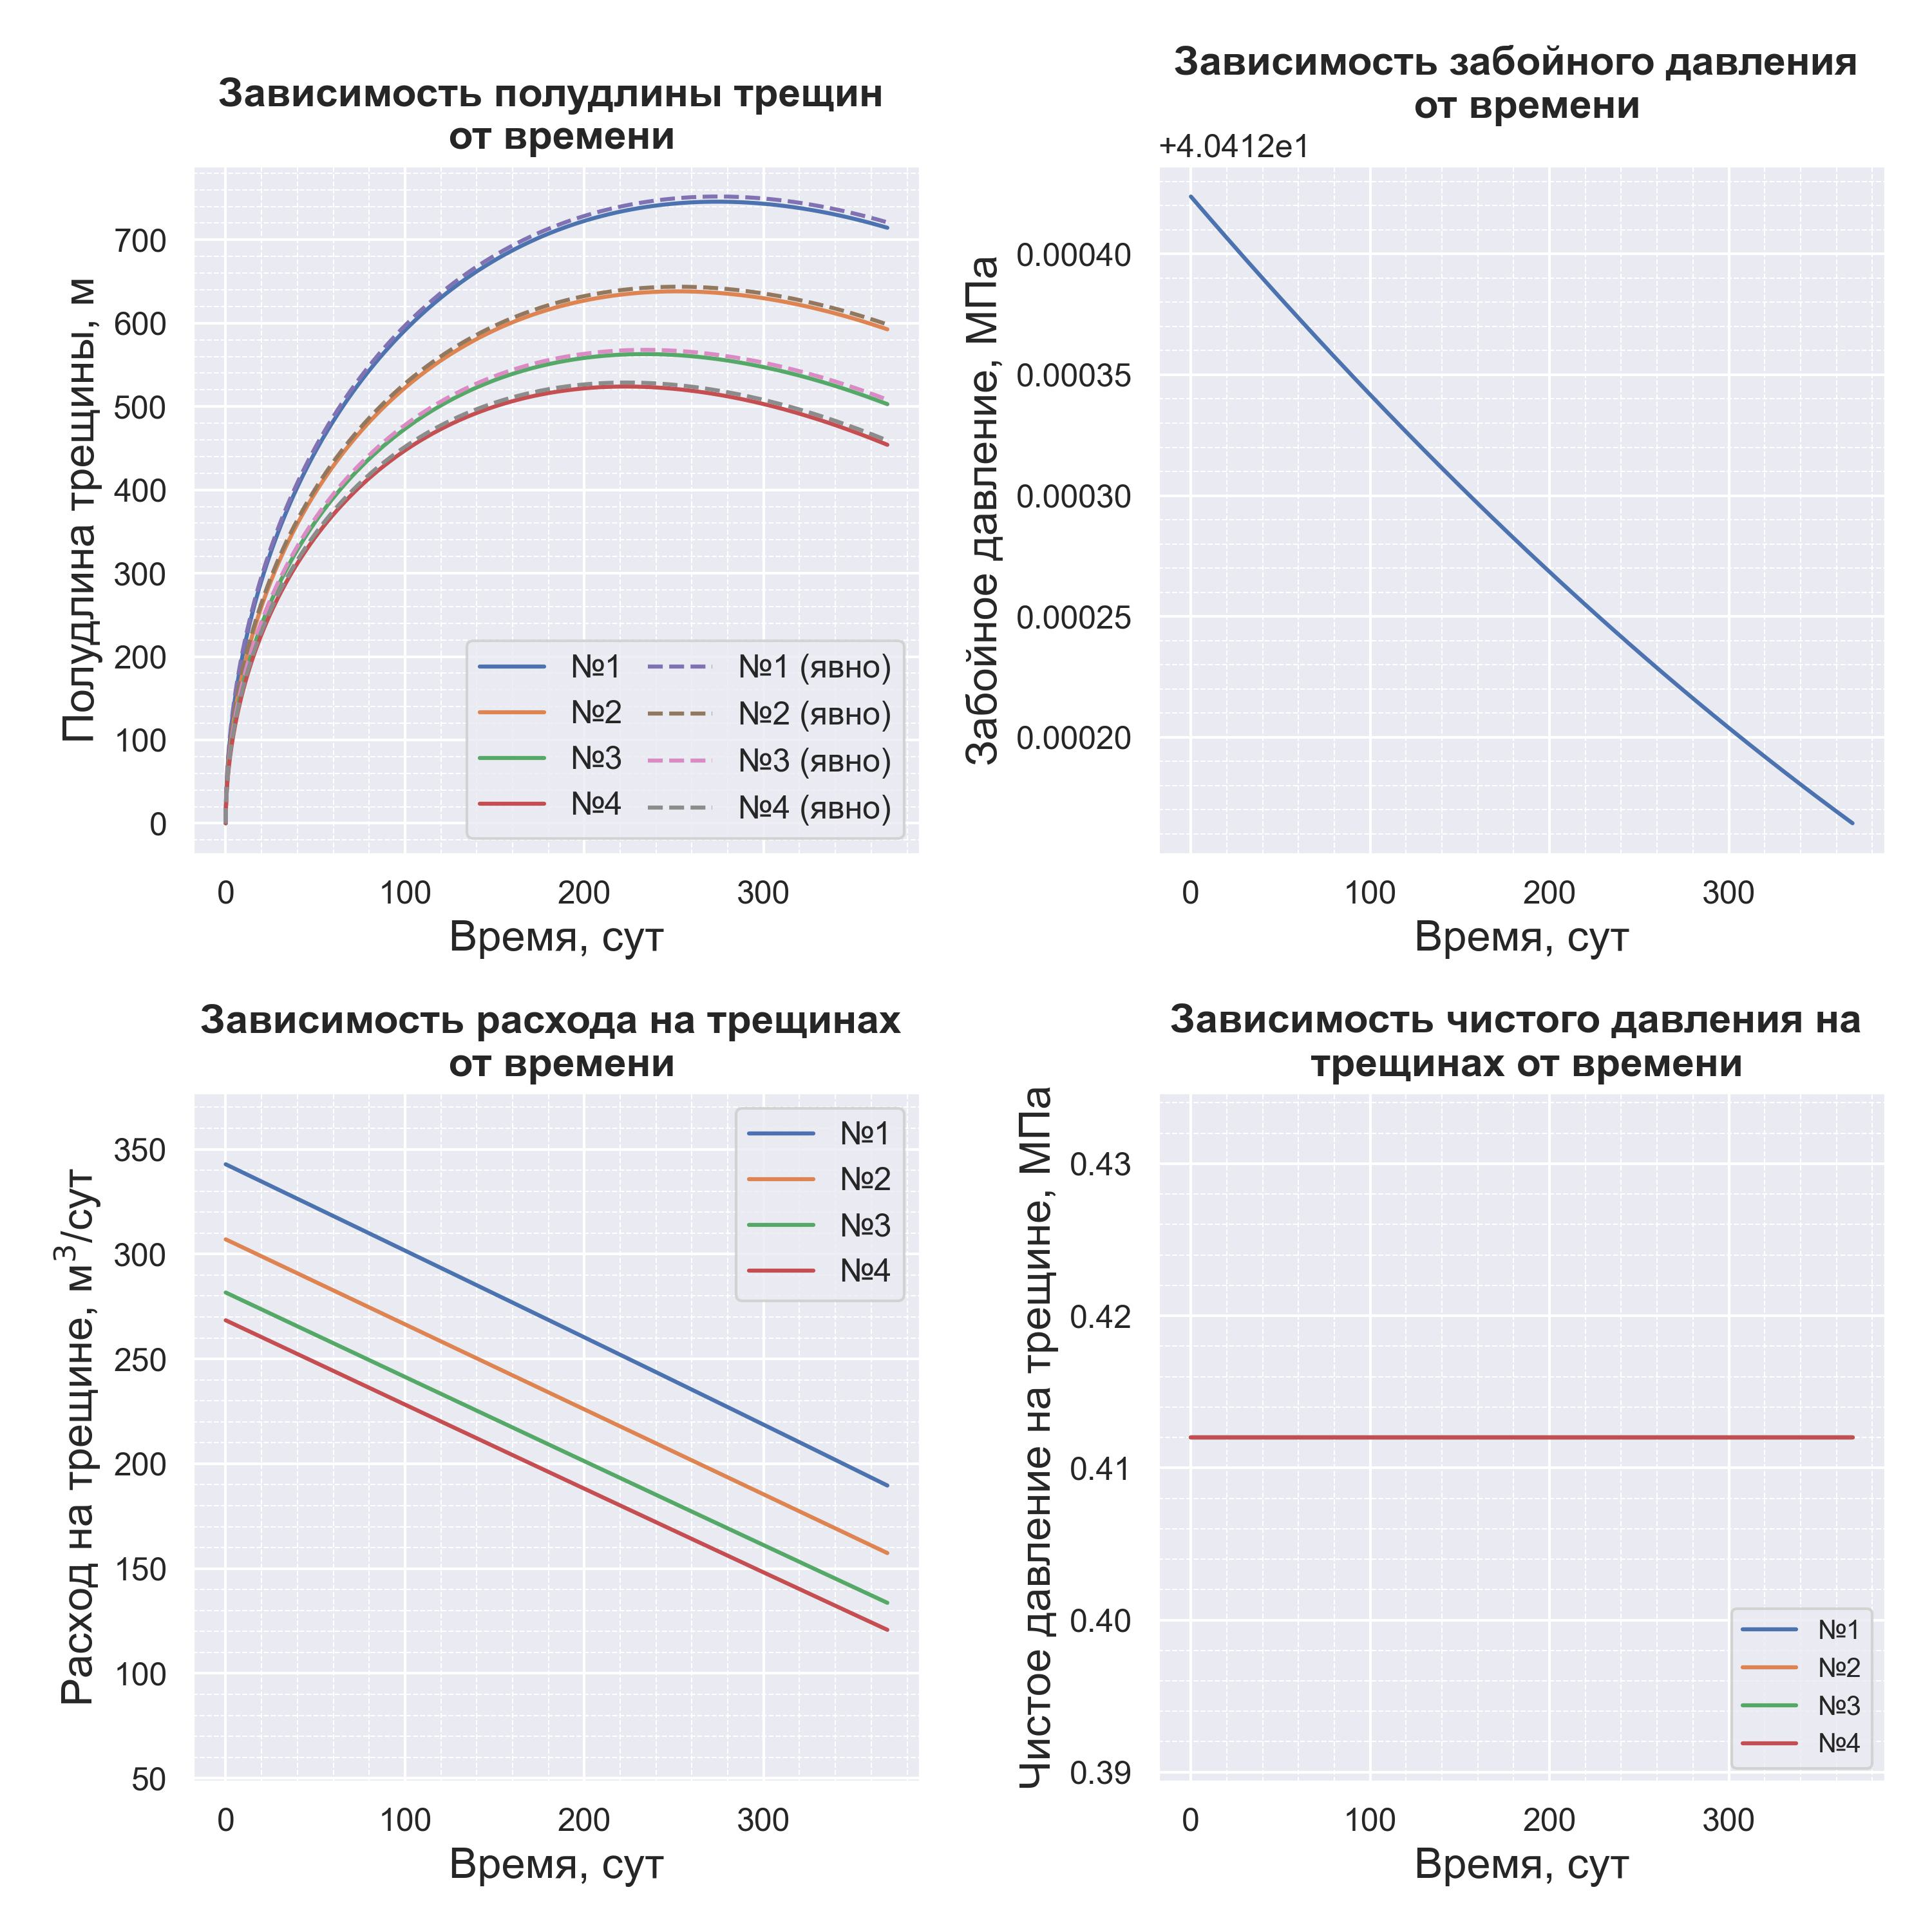
\includegraphics[width=\linewidth]{images/myimage5.jpg}
\caption{В случае одномерных утечек Картера и и линейном уменьшении расхода жидкости на забое скважины}
\label{fig:myimage5}
\end{figure}

При изменении качества перфораций.


При уменьшении горизонтальных напряжений пласта (за счёт термоупругого воздействия).


Для проверки работоспособности построенного алгоритма при большем количестве трещин проведён эксперимент в случае 6 трещин.



%
%\begin{figure}[H]
%	\adjustbox{minipage=1.3em,valign=t}{\subcaption{}\label{fig:p_0(q_0)}}%
%	\begin{subfigure}[t]{\dimexpr.5\linewidth-1.3em\relax}
%		\centering
%		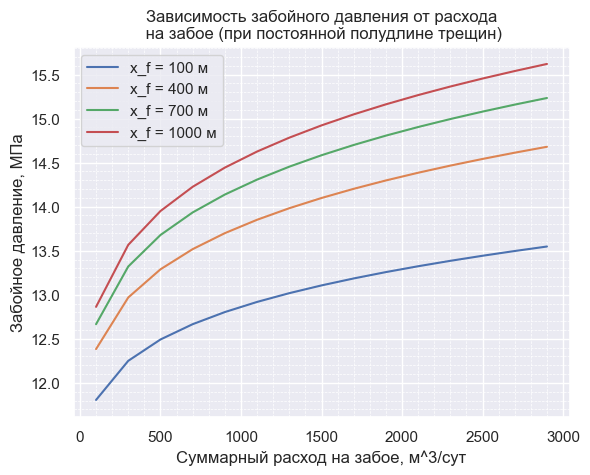
\includegraphics[width=.95\linewidth,valign=t]{images/p_0(q_0).png}
%	\end{subfigure}
%\hfill %выровнять по ширине
%	\adjustbox{minipage=1.3em,valign=t}{\subcaption{}\label{fig:p_0(x_f)}}%
%	\begin{subfigure}[t]{\dimexpr.5\linewidth-1.3em\relax}
%		\centering
%		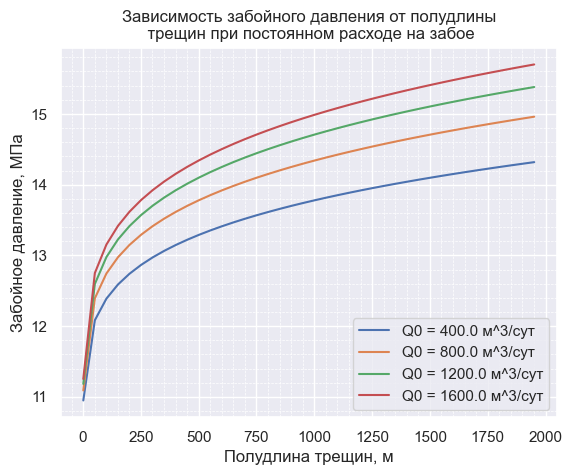
\includegraphics[width=.95\linewidth,valign=t]{images/p_0(x_f).png}
%	\end{subfigure}
%\captionsetup{justification=centering} %центрировать
%\caption{Зависимости забойного давления от основных параметров задачи: {\itshape a} --- от суммарного расхода на забое; {\itshape b} --- от полудлины трещин} 
%\label{fig:results1}
%\end{figure}

%Результаты моделирования представлены на рис. \ref{fig:results2}.
 
%\begin{figure}[H] 
%\center
%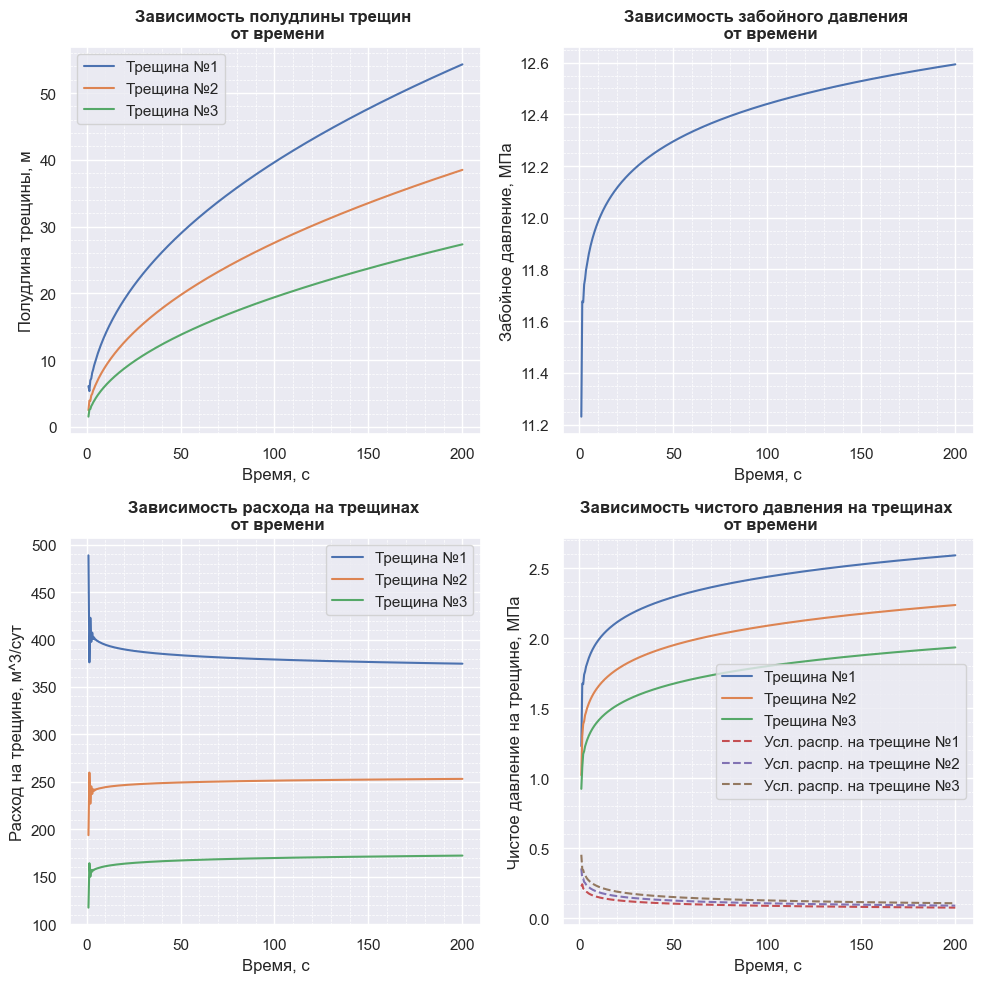
\includegraphics[width=.85\linewidth]{images/Kirchhoff+Koning.png}
%\caption{Результаты решения поставленной задачи} 
%\label{fig:results2}  
%\end{figure}

%В проведённом численном эксперименте трещины отличаются друг от друга количеством и диаметром перфораций.\newline
%У трещины 1: количество перфораций 32, диаметр перфораций 0.02 м.\newline
%У трещины 2: количество перфораций 2, диаметр перфораций 0.01 м.\newline
%У трещины 3: количество перфораций 1, диаметр перфораций 0.01 м.
%\\

%Код решения представлен по ссылке: \url{https://github.com/mualal/hydrofracturing/blob/master/notebooks/02_fractures_growth_with_Koning.ipynb}

%Из графиков на рис. \ref{fig:results2} видим, что большую часть потока забирает на себя трещина с лучшими перфорациями.
%Эта же трещина лидирует по скорости роста.

%Также видим, что при росте трещин требуется всё большее забойное давление для того, чтобы поддерживать этот рост.

%При выбранных входных параметрах построенной модели чистое давление в каждой из трещин существенно превышает давления критерия распространения, следовательно, при достаточно высоком забойном давлении все трещины будут расти одновременно.
